%% bare_conf.tex
%% V1.3
%% 2007/01/11
%% by Michael Shell
%% See:
%% http://www.michaelshell.org/
%% for current contact information.
%%
%% This is a skeleton file demonstrating the use of IEEEtran.cls
%% (requires IEEEtran.cls version 1.7 or later) with an IEEE conference paper.
%%
%% Support sites:
%% http://www.michaelshell.org/tex/ieeetran/
%% http://www.ctan.org/tex-archive/macros/latex/contrib/IEEEtran/
%% and
%% http://www.ieee.org/

%%*************************************************************************
%% Legal Notice:
%% This code is offered as-is without any warranty either expressed or
%% implied; without even the implied warranty of MERCHANTABILITY or
%% FITNESS FOR A PARTICULAR PURPOSE! 
%% User assumes all risk.
%% In no event shall IEEE or any contributor to this code be liable for
%% any damages or losses, including, but not limited to, incidental,
%% consequential, or any other damages, resulting from the use or misuse
%% of any information contained here.
%%
%% All comments are the opinions of their respective authors and are not
%% necessarily endorsed by the IEEE.
%%
%% This work is distributed under the LaTeX Project Public License (LPPL)
%% ( http://www.latex-project.org/ ) version 1.3, and may be freely used,
%% distributed and modified. A copy of the LPPL, version 1.3, is included
%% in the base LaTeX documentation of all distributions of LaTeX released
%% 2003/12/01 or later.
%% Retain all contribution notices and credits.
%% ** Modified files should be clearly indicated as such, including  **
%% ** renaming them and changing author support contact information. **
%%
%% File list of work: IEEEtran.cls, IEEEtran_HOWTO.pdf, bare_adv.tex,
%%                    bare_conf.tex, bare_jrnl.tex, bare_jrnl_compsoc.tex
%%*************************************************************************

% *** Authors should verify (and, if needed, correct) their LaTeX system  ***
% *** with the testflow diagnostic prior to trusting their LaTeX platform ***
% *** with production work. IEEE's font choices can trigger bugs that do  ***
% *** not appear when using other class files.                            ***
% The testflow support page is at:
% http://www.michaelshell.org/tex/testflow/



% Note that the a4paper option is mainly intended so that authors in
% countries using A4 can easily print to A4 and see how their papers will
% look in print - the typesetting of the document will not typically be
% affected with changes in paper size (but the bottom and side margins will).
% Use the testflow package mentioned above to verify correct handling of
% both paper sizes by the user's LaTeX system.
%
% Also note that the "draftcls" or "draftclsnofoot", not "draft", option
% should be used if it is desired that the figures are to be displayed in
% draft mode.
%
%\documentclass[conference]{IEEEtran}
% Add the compsoc option for Computer Society conferences.
%
% If IEEEtran.cls has not been installed into the LaTeX system files,
% manually specify the path to it like:
%\documentclass[conference]{/backup/home/diegolocal/Documents/Latex/IEEEtran}
\documentclass[conference]{IEEEtran}

\long\def\comment#1{} %%% to comment out a section of text

\long\def\comment#1{} %%% to comment out a section
\usepackage{xspace}
\newcommand{\ie}[0]{{\em i.e.}\ }
\newcommand{\eg}[0]{{\em e.g.}\ }
\newcommand{\etal}[0]{{\em et al.}\xspace }
\newcommand{\etc}[0]{{\em etc.}\xspace}
\newcommand{\vs}[0]{{\em vs.}\xspace}
\newcommand{\vv}[0]{{\em vice-versa}\xspace}

% Some very useful LaTeX packages include:
% (uncomment the ones you want to load)


% *** MISC UTILITY PACKAGES ***
%
%\usepackage{ifpdf}
% Heiko Oberdiek's ifpdf.sty is very useful if you need conditional
% compilation based on whether the output is pdf or dvi.
% usage:
% \ifpdf
%   % pdf code
% \else
%   % dvi code
% \fi
% The latest version of ifpdf.sty can be obtained from:
% http://www.ctan.org/tex-archive/macros/latex/contrib/oberdiek/
% Also, note that IEEEtran.cls V1.7 and later provides a builtin
% \ifCLASSINFOpdf conditional that works the same way.
% When switching from latex to pdflatex and vice-versa, the compiler may
% have to be run twice to clear warning/error messages.






% *** CITATION PACKAGES ***
%
\usepackage{cite}
% cite.sty was written by Donald Arseneau
% V1.6 and later of IEEEtran pre-defines the format of the cite.sty package
% \cite{} output to follow that of IEEE. Loading the cite package will
% result in citation numbers being automatically sorted and properly
% "compressed/ranged". e.g., [1], [9], [2], [7], [5], [6] without using
% cite.sty will become [1], [2], [5]--[7], [9] using cite.sty. cite.sty's
% \cite will automatically add leading space, if needed. Use cite.sty's
% noadjust option (cite.sty V3.8 and later) if you want to turn this off.
% cite.sty is already installed on most LaTeX systems. Be sure and use
% version 4.0 (2003-05-27) and later if using hyperref.sty. cite.sty does
% not currently provide for hyperlinked citations.
% The latest version can be obtained at:
% http://www.ctan.org/tex-archive/macros/latex/contrib/cite/
% The documentation is contained in the cite.sty file itself.



%
\usepackage{graphicx}  %added EN 2/22/12
%  \usepackage[pdftex]{graphicx}

% *** Commented out BH 2/3/15 because of "Option clash for package graphicx" error ***
%% *** GRAPHICS RELATED PACKAGES ***
%%
%\ifCLASSINFOpdf
%  \usepackage[pdftex]{graphicx}
%  % declare the path(s) where your graphic files are
%  % \graphicspath{{../pdf/}{../jpeg/}}
%  % and their extensions so you won't have to specify these with
%  % every instance of \includegraphics
%  % \DeclareGraphicsExtensions{.pdf,.jpeg,.png}
%\else
%  % or other class option (dvipsone, dvipdf, if not using dvips). graphicx
%  % will default to the driver specified in the system graphics.cfg if no
%  % driver is specified.
%  % \usepackage[dvips]{graphicx}
%  % declare the path(s) where your graphic files are
%  % \graphicspath{{../eps/}}
%  % and their extensions so you won't have to specify these with
%  % every instance of \includegraphics
%  % \DeclareGraphicsExtensions{.eps}
%\fi
%% graphicx was written by David Carlisle and Sebastian Rahtz. It is
%% required if you want graphics, photos, etc. graphicx.sty is already
%% installed on most LaTeX systems. The latest version and documentation can
%% be obtained at: 
%% http://www.ctan.org/tex-archive/macros/latex/required/graphics/
%% Another good source of documentation is "Using Imported Graphics in
%% LaTeX2e" by Keith Reckdahl which can be found as epslatex.ps or
%% epslatex.pdf at: http://www.ctan.org/tex-archive/info/
%%
%% latex, and pdflatex in dvi mode, support graphics in encapsulated
%% postscript (.eps) format. pdflatex in pdf mode supports graphics
%% in .pdf, .jpeg, .png and .mps (metapost) formats. Users should ensure
%% that all non-photo figures use a vector format (.eps, .pdf, .mps) and
%% not a bitmapped formats (.jpeg, .png). IEEE frowns on bitmapped formats
%% which can result in "jaggedy"/blurry rendering of lines and letters as
%% well as large increases in file sizes.
%%
%% You can find documentation about the pdfTeX application at:
%% http://www.tug.org/applications/pdftex





% *** MATH PACKAGES ***
%
%\usepackage[cmex10]{amsmath}
% A popular package from the American Mathematical Society that provides
% many useful and powerful commands for dealing with mathematics. If using
% it, be sure to load this package with the cmex10 option to ensure that
% only type 1 fonts will utilized at all point sizes. Without this option,
% it is possible that some math symbols, particularly those within
% footnotes, will be rendered in bitmap form which will result in a
% document that can not be IEEE Xplore compliant!
%
% Also, note that the amsmath package sets \interdisplaylinepenalty to 10000
% thus preventing page breaks from occurring within multiline equations. Use:
%\interdisplaylinepenalty=2500
% after loading amsmath to restore such page breaks as IEEEtran.cls normally
% does. amsmath.sty is already installed on most LaTeX systems. The latest
% version and documentation can be obtained at:
% http://www.ctan.org/tex-archive/macros/latex/required/amslatex/math/





% *** SPECIALIZED LIST PACKAGES ***
%
%\usepackage{algorithmic}
% algorithmic.sty was written by Peter Williams and Rogerio Brito.
% This package provides an algorithmic environment fo describing algorithms.
% You can use the algorithmic environment in-text or within a figure
% environment to provide for a floating algorithm. Do NOT use the algorithm
% floating environment provided by algorithm.sty (by the same authors) or
% algorithm2e.sty (by Christophe Fiorio) as IEEE does not use dedicated
% algorithm float types and packages that provide these will not provide
% correct IEEE style captions. The latest version and documentation of
% algorithmic.sty can be obtained at:
% http://www.ctan.org/tex-archive/macros/latex/contrib/algorithms/
% There is also a support site at:
% http://algorithms.berlios.de/index.html
% Also of interest may be the (relatively newer and more customizable)
% algorithmicx.sty package by Szasz Janos:
% http://www.ctan.org/tex-archive/macros/latex/contrib/algorithmicx/




% *** ALIGNMENT PACKAGES ***
%
%\usepackage{array}
% Frank Mittelbach's and David Carlisle's array.sty patches and improves
% the standard LaTeX2e array and tabular environments to provide better
% appearance and additional user controls. As the default LaTeX2e table
% generation code is lacking to the point of almost being broken with
% respect to the quality of the end results, all users are strongly
% advised to use an enhanced (at the very least that provided by array.sty)
% set of table tools. array.sty is already installed on most systems. The
% latest version and documentation can be obtained at:
% http://www.ctan.org/tex-archive/macros/latex/required/tools/


%\usepackage{mdwmath}
%\usepackage{mdwtab}
% Also highly recommended is Mark Wooding's extremely powerful MDW tools,
% especially mdwmath.sty and mdwtab.sty which are used to format equations
% and tables, respectively. The MDWtools set is already installed on most
% LaTeX systems. The lastest version and documentation is available at:
% http://www.ctan.org/tex-archive/macros/latex/contrib/mdwtools/


% IEEEtran contains the IEEEeqnarray family of commands that can be used to
% generate multiline equations as well as matrices, tables, etc., of high
% quality.


%\usepackage{eqparbox}
% Also of notable interest is Scott Pakin's eqparbox package for creating
% (automatically sized) equal width boxes - aka "natural width parboxes".
% Available at:
% http://www.ctan.org/tex-archive/macros/latex/contrib/eqparbox/





% *** SUBFIGURE PACKAGES ***
%\usepackage[tight,footnotesize]{subfigure}
% subfigure.sty was written by Steven Douglas Cochran. This package makes it
% easy to put subfigures in your figures. e.g., "Figure 1a and 1b". For IEEE
% work, it is a good idea to load it with the tight package option to reduce
% the amount of white space around the subfigures. subfigure.sty is already
% installed on most LaTeX systems. The latest version and documentation can
% be obtained at:
% http://www.ctan.org/tex-archive/obsolete/macros/latex/contrib/subfigure/
% subfigure.sty has been superceeded by subfig.sty.



%\usepackage[caption=false]{caption}
%\usepackage[font=footnotesize]{subfig}
% subfig.sty, also written by Steven Douglas Cochran, is the modern
% replacement for subfigure.sty. However, subfig.sty requires and
% automatically loads Axel Sommerfeldt's caption.sty which will override
% IEEEtran.cls handling of captions and this will result in nonIEEE style
% figure/table captions. To prevent this problem, be sure and preload
% caption.sty with its "caption=false" package option. This is will preserve
% IEEEtran.cls handing of captions. Version 1.3 (2005/06/28) and later 
% (recommended due to many improvements over 1.2) of subfig.sty supports
% the caption=false option directly:
\usepackage[caption=false,font=footnotesize]{subfig}
%
% The latest version and documentation can be obtained at:
% http://www.ctan.org/tex-archive/macros/latex/contrib/subfig/
% The latest version and documentation of caption.sty can be obtained at:
% http://www.ctan.org/tex-archive/macros/latex/contrib/caption/




% *** FLOAT PACKAGES ***
%
\usepackage{fixltx2e}
% fixltx2e, the successor to the earlier fix2col.sty, was written by
% Frank Mittelbach and David Carlisle. This package corrects a few problems
% in the LaTeX2e kernel, the most notable of which is that in current
% LaTeX2e releases, the ordering of single and double column floats is not
% guaranteed to be preserved. Thus, an unpatched LaTeX2e can allow a
% single column figure to be placed prior to an earlier double column
% figure. The latest version and documentation can be found at:
% http://www.ctan.org/tex-archive/macros/latex/base/



%\usepackage{stfloats}
% stfloats.sty was written by Sigitas Tolusis. This package gives LaTeX2e
% the ability to do double column floats at the bottom of the page as well
% as the top. (e.g., "\begin{figure*}[!b]" is not normally possible in
% LaTeX2e). It also provides a command:
%\fnbelowfloat
% to enable the placement of footnotes below bottom floats (the standard
% LaTeX2e kernel puts them above bottom floats). This is an invasive package
% which rewrites many portions of the LaTeX2e float routines. It may not work
% with other packages that modify the LaTeX2e float routines. The latest
% version and documentation can be obtained at:
% http://www.ctan.org/tex-archive/macros/latex/contrib/sttools/
% Documentation is contained in the stfloats.sty comments as well as in the
% presfull.pdf file. Do not use the stfloats baselinefloat ability as IEEE
% does not allow \baselineskip to stretch. Authors submitting work to the
% IEEE should note that IEEE rarely uses double column equations and
% that authors should try to avoid such use. Do not be tempted to use the
% cuted.sty or midfloat.sty packages (also by Sigitas Tolusis) as IEEE does
% not format its papers in such ways.





% *** PDF, URL AND HYPERLINK PACKAGES ***
%
%\usepackage{url}
% url.sty was written by Donald Arseneau. It provides better support for
% handling and breaking URLs. url.sty is already installed on most LaTeX
% systems. The latest version can be obtained at:
% http://www.ctan.org/tex-archive/macros/latex/contrib/misc/
% Read the url.sty source comments for usage information. Basically,
% \url{my_url_here}.





% *** Do not adjust lengths that control margins, column widths, etc. ***
% *** Do not use packages that alter fonts (such as pslatex).         ***
% There should be no need to do such things with IEEEtran.cls V1.6 and later.
% (Unless specifically asked to do so by the journal or conference you plan
% to submit to, of course. )


% correct bad hyphenation here
\hyphenation{op-tical net-works semi-conduc-tor}


\begin{document}
%
% paper title
% can use linebreaks \\ within to get better formatting as desired
\title{A neural model for perceptual \\ organization of 3D surfaces}

% author names and affiliations
% use a multiple column layout for up to three different
% affiliations
\author{\IEEEauthorblockN{Brian Hu, R\"udiger von
  der Heydt, Ernst Niebur}
\IEEEauthorblockA{Zanvyl Krieger Mind/Brain Institute\\Johns Hopkins University\\
Baltimore, Maryland 21218}
}

% conference papers do not typically use \thanks and this command
% is locked out in conference mode. If really needed, such as for
% the acknowledgment of grants, issue a \IEEEoverridecommandlockouts
% after \documentclass

% for over three affiliations, or if they all won't fit within the width
% of the page, use this alternative format:
% 
%\author{\IEEEauthorblockN{Michael Shell\IEEEauthorrefmark{1},
%Homer Simpson\IEEEauthorrefmark{2},
%James Kirk\IEEEauthorrefmark{3}, 
%Montgomery Scott\IEEEauthorrefmark{3} and
%Eldon Tyrell\IEEEauthorrefmark{4}}
%\IEEEauthorblockA{\IEEEauthorrefmark{1}School of Electrical and Computer Engineering\\
%Georgia Institute of Technology,
%Atlanta, Georgia 30332--0250\\ Email: see http://www.michaelshell.org/contact.html}
%\IEEEauthorblockA{\IEEEauthorrefmark{2}Twentieth Century Fox, Springfield, USA\\
%Email: homer@thesimpsons.com}
%\IEEEauthorblockA{\IEEEauthorrefmark{3}Starfleet Academy, San Francisco, California 96678-2391\\
%Telephone: (800) 555--1212, Fax: (888) 555--1212}
%\IEEEauthorblockA{\IEEEauthorrefmark{4}Tyrell Inc., 123 Replicant Street, Los Angeles, California 90210--4321}}




% use for special paper notices
%\IEEEspecialpapernotice{(Invited Paper)}




% make the title area
\maketitle


\begin{abstract}
%\boldmath
Perceptual organization is the process by which the visual scene is
structured into coherent units suitable for further processing and
selection. Having been primarily studied in 2D, here we present a
neural model for perceptual organization of 3D surfaces. We
demonstrate that our model is able to reproduce several key
psychophysical results, including the spread of visual attention across 3D
surfaces. 
\end{abstract}
% IEEEtran.cls defaults to using nonbold math in the Abstract.
% This preserves the distinction between vectors and scalars. However,
% if the conference you are submitting to favors bold math in the abstract,
% then you can use LaTeX's standard command \boldmath at the very start
% of the abstract to achieve this. Many IEEE journals/conferences frown on
% math in the abstract anyway.

% no keywords




% For peer review papers, you can put extra information on the cover
% page as needed:
% \ifCLASSOPTIONpeerreview
% \begin{center} \bfseries EDICS Category: 3-BBND \end{center}
% \fi
%
% For peerreview papers, this IEEEtran command inserts a page break and
% creates the second title. It will be ignored for other modes.
\IEEEpeerreviewmaketitle



\section{Introduction}
% no \IEEEPARstart
Since we live in a complex 3D world, competent interaction with the
surrounding 3D scene structure is indispensable to us and our
machines. Access to information about
surfaces present in the scene allows us to perform a wide variety of
tasks, ranging from motor planning (\eg reaching for a cup a certain
distance away on the table) to spatial navigation (\eg following
directions in a new city environment).

%While it may be tempting to believe that only "higher" organisms need to have a representation of 3D scene structure, similar abilities have also been found in much "simpler" animals. For example, jumping spiders hunt for prey in complex 3D environments. Their behavior consists of first analyzing the 3D surface layout of the environment before planning and executing a route to their prey. Jumping spiders must keep track of their movement goal despite large changes in their own position within the 3D environment, pointing to a stable and persistent surface representation. These studies illustrate that the representation of surfaces within 3D scenes may be an ecologically important function, conserved across many different animal species and adapted to their own natural environments.

In studying perceptual organization, researchers have traditionally
relied on simple 2D stimuli such as oriented
bars~\cite{Palmer_02}. Results from these studies provide support for
the importance of well-known Gestalt principles~\cite{Koffka35,
  Wertheimer23}, for instance 
that visual elements are grouped together in a way that
begins to give meaning to the visual scene (\eg figure
\vs background). However, it is unclear how well the results from
these relatively simple experiments generalize to the 3D objects and
scenes regularly encountered in natural settings. Because we act in a
3D world, perceptual organization must also help to arrange 3D
information in a way that can guide our actions. 

Perceptual organization also provides a structure for selectively
attending to groups of objects~\cite{Treisman_Gelade80}. Supported by
extensive psychophysical data, Nakayama, He, and
Shimojo~\cite{Nakayama_etal95} proposed that surface representations
play a key role in intermediate-level vision. For example, by
selectively attending to a surface in 3D space, subjects can perform
efficient search for a conjunction
target~\cite{Nakayama_Silverman86}. In a separate cueing experiment,
attention was shown to spread automatically across
surfaces~\cite{He_Nakayama95}. These abilities indicate powerful
mechanisms for grouping objects into surfaces in 3D space, and suggest
that structuring the world in terms of surfaces might be an
ecologically important function. These results also have implications
for the internal representation of surfaces, because they imply that
the visual scene is processed in a way that preserves its 3D
structure. This representation must also be able to bring together
information from different sensory modalities (\eg vision, audition,
\etc), in order to form a common representation of the 3D environment
that is useful for an agent's behavioral goals~\cite{Lewicki_etal14}.

In addition to being studied by human psychophysical approaches,
perceptual organization has been the subject of many studies in the
visual system of non-human primates. Many neurons in early visual cortex encode the side to which an object
border belongs, a phenomenon known as border
ownership~\cite{Zhou_etal00}. Selectivity for the side of ownership
involves integrating global context information about the
object. Several models have been proposed~\cite{Zhaoping05,
  Craft_etal07} to describe how a neuron's border ownership
selectivity can be modulated by visual input far away from its
classical receptive field with the observed high specificity of object details. % %bh this phrase is a little confusing to me?
One
view is that this contextual input is provided by feedback connections
from ``grouping cells''~\cite{Craft_etal07} which bias the activity of
border ownership cells and thus generate their context-dependent
responses. Mihalas et al.~\cite{Mihalas_etal11b} have also shown that
grouping cells can direct and sharpen a broad attentional spotlight to
the lower-level features of a specific object. In the present study,
we extend this grouping framework to 3D space to show how oriented 3D
elements can be grouped into planar surfaces.

Currently, we know very little about how surfaces are represented in
the brain, and how this representation is computed.  Our model sheds
light on a possible neural representation of 3D surfaces and relates
this model to previous psychophysical results.

\begin{figure} [h!]
\centering
\vspace{-10pt}
\includegraphics[width=3 in]{figs/groupingcircuit}
\caption{Network structure (adapted from ref.~\cite{Marshall_etal96}).}
\label{NetworkStructure}
\end{figure}

\section{Methods}
An overview of the network structure of our model is shown in
Figure~\ref{NetworkStructure}. We extend a neural model of visual
stereomatching~\cite{Marshall_etal96} that is conceptually similar to
grouping models previously proposed for 2D stimuli~\cite{Craft_etal07,
  Mihalas_etal11b, Russell_etal14}.  The model contains three layers
of neurons. The first layer consists of monocular cells, which respond
to visual features (e.g. spots, edges, {\em etc.}) presented to either
the left or right eye. The input to the model consists of pairs of
stereo images, as would be seen by the left and right eyes. In our
model, we set the image input to a value of unity wherever a stimulus is present and zero elsewhere.
%en unclear. 
%bh is this a little easier to understand?
%en no, it is not clear what you mean  by 'set input to unity'. Do you
%mean it is unity where a stimulus is present and zero elsewhere?
%bh yes this is what I mean- thanks! I hope it is clear now.

The second layer consists of binocular cells, which receive excitatory
input from monocular cells. These cells are tuned
to a certain disparity based on a fixed spatial weighting between the
left and right monocular cells, analogous to the disparity-selective
binocular neurons in visual cortex of
monkeys~\cite{Poggio_Fischer77, Poggio_Poggio84} and
cats~\cite{Bishop_Pettigrew86, Ohzawa_etal90}. Lateral inhibition
between cells representing different disparities along the same left-
or right-eye line of sight reduces potential false matches~\cite{Marr_Poggio76}.

The third and final layer consists of planar grouping cells which
receive excitatory input from populations of disparity-selective
cells. Receptive fields of the planar grouping cells are relatively broad and non-specific, resembling surface patches with a certain range of depth and orientation selectivity in 3D space.
These cells may correspond to neurons found 
in parietal cortex, which have been shown to be selective for the tilt
and slant of planar surfaces~\cite{Rosenberg_etal13}. In our model, we
used a total of 15~planar grouping cells, which was sufficient to ``tile''
the whole 3D visual scene. Planar grouping cells compete with each
other through lateral inhibition, which helps to select the best
possible interpretation of surfaces within the scene. Additionally,
planar grouping cells send reciprocal feedback connections to the
disparity-selective cells that define their surface, akin to the
relationship between grouping cells and border ownership cells in
models of 2D scenes~\cite{Craft_etal07,Mihalas_etal11b}. To avoid
uncontrolled feedback excitation, feedback is multiplicative and only amplifies existing feedforward excitation.
Selective attention is modeled as an additive input to those planar
grouping neurons representing attended objects. This attentional
modulation input is set to a value of 0.25 of the sensory input.

All model neurons are simulated as single compartment units with an
activity that is modeled as a continuous variable (rate coding). These
units are zero-threshold, linear neurons which receive excitatory and
inhibitory current inputs. The activity of the units is determined by
a set of coupled, first-order nonlinear ordinary differential
equations, which can be solved in MATLAB (MathWorks)
using standard numerical integration methods (Euler, Runge-Kutta,
\etc) 

\begin{figure}[h!]
\centering
\includegraphics[width=3in]{figs/nakayama}
\caption{Psychophysical and model results (adapted from
  ref~\cite{He_Nakayama95}). For each trial type (A or B), the top row
  shows the different stimuli, the middle row
  shows representative reaction times, and the bottom row shows the
  degree of attentional modulation of disparity-selective cells on the
  attended plane. Increase in activity is assumed to be inversely
  proportion to reaction times.} 
\vspace{-11pt}
\label{ModelResults}
\end{figure}

\section{Results}
Figure~\ref{ModelResults} illustrates the experimental paradigm of He
and Nakayama \cite{He_Nakayama95}.
In Figure~\ref{ModelResults}A, subjects
had to search for the odd-colored target in the middle depth
plane; planes are outlined by rectangles that were not visible to the observers. The target was unique in
this search plane but visually identical distractors
 were present in other depth
planes. In A-a, objects are aligned with the search plane while in A-b
and A-c, they are slanted out of the plane. The
middle row in A shows measured reaction times for three different
numbers of distractors.
%took out comment about number of distractors because the x axis is actually chopped off (doesn't show the number of distractors) and we don't comment any further on it/it is not needed to understand results
%en but we need to explain what is shown in the figure! We cannot just
%show 3 columns without saying what they are
% bh re-added your line about the different number of distractors
They are significantly shorter when the objects are coplanar with the search plane (A-a) compared to when they are not aligned with the plane (A-b and A-c).

\begin{figure}[h!]
\centering
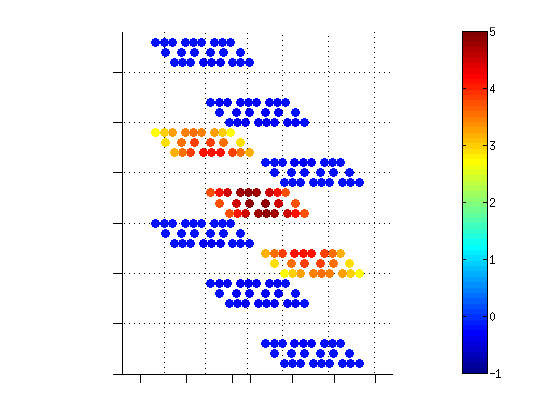
\includegraphics[width=3in]{figs/attentionmod}
\caption{Spread of attention across surfaces. When attention is
  directed to the center slanted plane (as in the experiment in Figure
  2B-a), attention enhances the activity of all cells along the
  surface (red), while suppressing the activity of cells belonging to
  other surfaces (blue).} 
\vspace{-11pt}
\label{ModelResults2}
\end{figure}

In our model, we assume that the visual system can selectively direct
attention towards a specific surface 
by providing additional excitatory input to the grouping cell
that represents this surface. As shown in Figure~\ref{NetworkStructure},
activity from the grouping cell selectively feeds back to all
objects on that surface. In the case of Figure~\ref{ModelResults}A-a, the grouping cell corresponding to the middle fronto-parallel plane receives this attentional input. 
Activation of the disparity-selective cells in the search
plane, shown in Figure~\ref{ModelResults}A-a, bottom row, is thus
high. Among the objects in the
search plane, the target has a unique color, which results in
efficient search and the target being identified immediately. Reaction
times are difficult to simulate in detail, therefore 
the increase in mean activity of disparity-selective cells on the
attended plane due to attentional modulation is plotted instead,
which is assumed to be inversely proportional to reaction times. The
high activation level, bottom row, translates thus into short reaction
times, middle row.

In contrast, in
Figure~\ref{ModelResults}A-b, the search plane is no longer a
well-formed surface but contains objects that are slanted
backwards. Directing attention to the middle fronto-parallel plane
then has little effect on the disparity-selective cells in the search
plane. 
%executed in a plane (the middle fronto-parallel plane) that is
%different from the planes in which the figure elements are grouped
%(the three horizontal planes).
%
%bh I think herein lies the confusion? In the experiment, although
%Figure 2A-b looks like three horizontal planes, they were actually
%just slanted backwards. So, it is actually more similar to Figure
%2A-c in that no well-defined surfaces were present in the scene, but
%the task required attending to the middle search plane. The longer
%reaction times is because you cannot attend to the surface formed by
%the elements as in 2A-a (which would give you pop-out), and you have
%to do serial search through each element in the search plane 
%en Yes, that explains it! 
%I will leave this comment here in the text, in case I forget it again!
 Search therefore cannot occur entirely
within a single plane of coplanar, grouped elements and becomes inefficient, with
much higher reaction times (middle row). These long reaction times are
reflected in the low activation level of the disparity-selective cells
(bottom row). Figure~\ref{ModelResults}A-c shows the analog result for
figure elements that are slanted forward rather than backwards, as in
A-b. Again, reaction times are long and population
activity is low. 

The result is not restricted to fronto-parallel planes, as similar
reaction time results were also found for slanted planes in
Figure~\ref{ModelResults}B. When subjects are instructed to search in
a plane that is coplanar with the orientation of the figure elements
(middle plane in B-a), search is fast (B-a, middle row). In contrast,
when the figure elements do not align with the search plane (top
row in B-b and B-c), reaction time is increased (middle row).  Again,
under the assumption that reaction times are inversely related to
reaction times, the model reproduces human behavior (bottom row).

Attention to grouping neurons is then able to select sets of objects
organized in planes. Reaction times were fastest when 
the search array was a well-formed surface defined by locally
coplanar elements. When search array elements were slanted away
from this surface, reaction times increased. These results
suggest that attention is linked to and spreads across perceived
surfaces, which organize the visual scene
(Figure~\ref{ModelResults2}). 

\section{Conclusion}
Using a simple model of perceptual organization in 3D,  we are able to reproduce
psychophysical results from a visual search task that required
allocation of selective attention to surfaces within the scene. The
same grouping cells which organize the scene into planes also act as
``handles'' for top-down selective attention, enhancing the activity 
of coplanar elements belonging to the plane. Competition between
grouping cells results in surface enhancement of the plane
corresponding to the attended grouping cell, and suppression of other
planes within the scene. Our proposed surface representation aids
visual processing by providing a critical link between low-level
visual features and high-level object representations. 

% conference papers do not normally have an appendix


% use section* for acknowledgement
\section*{Acknowledgment}
This work is supported by the Office of Naval Research grant
N000141010278, the National Institutes of Health grant
R01EY016281-02, and the Visual Neuroscience Training Program fellowship (T32EY07143). %only one NIH grant allowed now.

% manually trigger a \newpage just before the given reference
% number - used to balance the columns on the last page
% adjust value as needed - may need to be readjusted if
% the document is modified later
%\IEEEtriggeratref{2}
% The "triggered" command can be changed if desired:
%\IEEEtriggercmd{\enlargethispage{-5in}}

%\newpage %instead of the trigger thing  --EN 2/2/3/12

% references section

% can use a bibliography generated by BibTeX as a .bbl file
% BibTeX documentation can be easily obtained at:
% http://www.ctan.org/tex-archive/biblio/bibtex/contrib/doc/
% The IEEEtran BibTeX style support page is at:
% http://www.michaelshell.org/tex/ieeetran/bibtex/
%\bibliographystyle{IEEEtran}
% argument is your BibTeX string definitions and bibliography database(s)
%\bibliography{IEEEabrv,../bib/paper}
%
% <OR> manually copy in the resultant .bbl file
% set second argument of \begin to the number of references
% (used to reserve space for the reference number labels box)
%\begin{thebibliography}{15}

\bibliographystyle{IEEEtran}
\bibliography{niebase}

%%en everything within \comment{} is commented out
%\comment{
%\bibliography{bib,bib/CraftModel,%
%bib/FahleFiguralBinding,%
%bib/FeldmanShape,%
%bib/FeldmanFG,%
%bib/BlumMAT,%
%bib/SakaiModel,%
%bib/IrvingHigherLevelTheory,%
%bib/JuleszKovacsNature,%
%bib/LeeV1MedialAxis1,%
%bib/LeeV1MedialAxis2,%
%bib/MATApps,%
%bib/LiFGEffects,%
%bib/MarrNishihara3D,%
%bib/SidiqShocks,%
%bib/ZhouBO}
%}
%\end{thebibliography}




% that's all folks
\end{document}
This is never printed. It switches the display to PDF rather than DVI.
%%% Local Variables:
%%% mode: latex
%%% TeX-PDF-mode: t
%%% End:
